\documentclass[11pt]{article}
\usepackage{std}

\title{COMP4680 Notes}
\author{Jeff Li}
\date{2023 S2}

\begin{document}

\maketitle

\setcounter{section}{-1}
\section{Introduction} 
A mathematical optimisation problem requires us to minimize an objective function $f_0(x)$, subject to constraint functions $f_i(x) \leq b_i$ for $i = 1, \ldots, m$. \par
A solution, or optimal point, $x^*$, has the smallest value of $f_0$ among all vectors that satisfy the constraints. \par 
There are three main types of problems which can be solved to different extents: 
\subsection{Least-squares Problems} 
Least-squares problems attempt to minimize $\norm{Ax - b}_2^2$ for some matrix $A$ and vector $b$. \par
There exists an analytical solution $x^* = (A^TA)^{-1}A^Tb$, there are reliable and efficient algorithms with computation time $O(n^2k)$ when $A \in \mathbb{R}^{k\times n}$, less if $A$ satisfies certain structures. 
\subsection{Convex Optimization Problems} 
Convex optimization problems are optimization problems where both the objective and constraint functions are convex, and is a superset of least-squares problems. \par 
There is no analytical solution, but there are algorithms with computation time $\mathrm{max}(O(n^3), \\O(n^2m), F)$ where $F$ is the cost of evaluating $f_i$'s and their second derivatives. 
\subsection{Nonconvex Optimization Problems} 
There is no general way to solve nonconvex optimization problems: they all involve some kind of compromise. \par
We may use local optimization methods (nonlinear programming), which is fast and finds a local minima around an initial guess, but may not be the global minima. \par
Or we may use global optimization methods, which finds the global solution but requires exponential time complexity. 

\newpage


\section{Preliminaries} 
\subsection{Sets}
A set, denoted as $S = \left\{ a_1, \ldots, a_n \right\}$, is a collection of distinct objects. \par
Some common notations: 
\begin{itemize}
    \item $a \in S$ denotes $a$ is an element of $S$
    \item $S \subseteq T$ denotes $S$ is a subset of $T$, that is, every element of $S$ is also an element of $T$
    \item $S \cup T$ denotes the union of $S$ and $T$, that is, the set of all elements that are in $S$ or $T$
    \item $S \cap T$ denotes the intersection of $S$ and $T$, that is, the set of all elements that are in both $S$ and $T$
    \item $S \times T$ denotes the Cartesian product of $S$ and $T$, that is, the set of all ordered pairs $(s, t)$ where $s \in S$ and $t \in T$
    \item $S \setminus T$ denotes the set difference of $S$ and $T$, that is, the set of all elements that are in $S$ but not in $T$
\end{itemize}  
Some common sets: 
\begin{itemize}
    \item $\mathbb{R}$ is the set of real numbers
    \item $\mathbb{R}^n$ is the set of $n$-dimensional real vectors
    \item $\mathbb{R}^{m\times n}$ is the set of $m \times n$ real matrices
    \item $\mathbb{C}$ is the set of complex numbers
    \item $\mathbb{Z}$ is the set of integera
    \item $\mathbb{R}_+$ is the set of nonnegative real numbers
    \item $\mathbb{R}_{++}$ is the set of positive real numbers
    \item $\emptyset$ is the empty set 
    \item $[a, b]$ is the closed interval from $a$ to $b$ (i.e. $\left\{ x \in \mathbb{R} \mid a \leq x \leq b \right\}$)
    \item $(a, b)$ is the open interval from $a$ to $b$ (i.e. $\left\{ x \in \mathbb{R} \mid a < x < b \right\}$)
    \item $[a, b)$ and $(a, b]$ are half-open intervals, defined similarly
\end{itemize}

\subsubsection*{Open and Closed Sets}
A subset $S \subseteq \mathbb{R}$ is \textbf{open} if for every $x \in S$, there exists $\epsilon > 0$ such that \\
\-\quad if $\norm{y - x}_2 < \epsilon$, then $y \in S$. \par
A subset $S \subseteq \mathbb{R}$ is \textbf{closed} if its complement $\mathbb{R} \setminus S$ is open. \par
A subset $S \subseteq \mathbb{R}$ is \textbf{bounded} if there exists $M > 0$ such that $\norm{a-b}_2 \leq M$ for all $a, b \in S$. \par

\subsubsection*{Infimum and Supremum}
The \textbf{infimum} of a set $S \subseteq \mathbb{R}$, written as $\mathrm{inf}(S)$, is the largest $y \in \mathbb{R}$ such that $y \leq x$ for all $x \in S$. If no such $y$ exists, we say $\mathrm{inf}(S) = -\infty$. \par
The \textbf{supremum} of a set $S \subseteq \mathbb{R}$, written as $\mathrm{sup}(S)$, is the smallest $y \in \mathbb{R}$ such that $y \geq x$ for all $x \in S$. If no such $y$ exists, we say $\mathrm{sup}(S) = \infty$. \par
We define $\mathrm{inf}(\emptyset) = \infty$ and $\mathrm{sup}(\emptyset) = -\infty$. \par 

\subsection{Functions} 
A function $f: A \rightarrow B$ is a mapping from its \textbf{domain} $A$ to its \textbf{codomain} $B$. \par
If $U \subseteq A$ and $V \subseteq B$, we define the \textbf{image} of $U$ under $f$ as $f(U) = \left\{ f(x) \mid x \in U \right\} \subseteq B$, and the \textbf{preimage} of $V$ under $f$ as $f^{-1}(V) = \left\{ x \in A \mid f(x) \in V \right\} \subseteq A$. \par

\subsection{Vector Spaces} 
A vector space $V$ is a set with two operations, vector addition and scalar multiplication, that satisfy the following axioms: 
\begin{itemize}
    \item $x + y = y + x$ (commutativity of vector addition)
    \item $(x + y) + z = x + (y + z)$ (associativity of vector addition)
    \item $x + \vec{0} = x$ (additive identity)
    \item $\forall x \in V, \exists y \in V$ such that $x + y = 0$, we write $y$ as $-x$ (additive inverse)
    \item $\alpha(x + y) = \alpha x + \alpha y$ (right distributivity)
    \item $(\alpha + \beta)x = \alpha x + \beta x$ (left distributivity)
    \item $1x = x$ (multiplicative identity)
\end{itemize}
We define the \textbf{zero vector} as a vector with all elements equal to 0, and the \textbf{ones vector} as a vector with all elements equal to 1. 

\subsubsection*{Euclidean Norm}
The Euclidean norm of a vector $\vec{v} = (v_1, \ldots, v_n)$ is 
\[ \norm{\vec{v}}_2 = \sqrt{v_1^2 + v_2^2 + \cdots + x_n^2} \] 
$\norm{\vec{v}}_2$ measures the length of $\vec{v}$. \par 
The norm satisfies: 
\begin{itemize}
    \item $\norm{\alpha\vec{v}} = \abs{\alpha}\norm{\vec{v}}$
    \item $\norm{\vec{u} + \vec{v}} \leq \norm{\vec{u}} + \norm{\vec{v}}$ (triangle inequality)
    \item $\norm{\vec{v}} \geq 0$ and $\norm{\vec{v}} = 0$ if and only if $\vec{v} = \vec{0}$ (positive definiteness)
\end{itemize}
There are other norms such as $\norm{\phantom{~.~}}_1$ and $\norm{\phantom{~.~}}_\infty$. 

\subsubsection*{Inner Products}
The inner product of two vectors $\vec{u} = (u_1, \ldots, u_n)$ and $\vec{v} = (v_1, \ldots, v_n)$ is defined by 
\[ \langle \vec{u}, \vec{v} \rangle = u_1v_1 + u_2v_2 + \cdots + u_nv_n. \] 
The inner product satisfies:
\begin{itemize}
    \item $\langle \alpha\vec{u}, \vec{v} \rangle = \alpha\langle \vec{u}, \vec{v} \rangle$
    \item $\langle \vec{u}_1 + \vec{u}_2, \vec{v} \rangle = \langle \vec{u}_1, \vec{v} \rangle + \langle \vec{u}_2, \vec{v} \rangle$
    \item $\langle \vec{u}, \vec{v} \rangle = \langle \vec{v}, \vec{u} \rangle$
    \item $\langle \vec{v}, \vec{v} \rangle = \norm{\vec{v}}_2^2$
\end{itemize}

\subsubsection*{Subspaces} 
A subspace of a vector space is a subset of the vector space that is also a vector space. \par
\subsubsection*{Independence}
A set of vectors $v_1, \ldots, v_n$ is (linearly) independent if and only if $\alpha_1v_1 + \cdots + \alpha_nv_n = 0$ implies $\alpha_1 = \cdots = \alpha_n = 0$. \par 
Conversely, if a set of vectors is linearly dependent, we can write one of the vectors as a linear combination of the others. \par
\subsubsection*{Bases}
The set of vectors $\left\{ v_1, \ldots, v_n \right\}$ form a basis of a vector space $V$ if 
\begin{itemize}
    \item they are linearly independent
    \item they span $V$, that is, every vector in $V$ can be written as a linear combination of the vectors in the set
\end{itemize}  
Equivalently, $\left\{ v_1, \ldots, v_n \right\}$ form a basis for $V$ if every $v \in V$ can be uniquely expressed as $v = \alpha_1v_1 + \cdots + \alpha_nv_n$. \par
We define the \textbf{dimension} of a vector space $V$ to be the number of vectors in any basis of $V$. \par
The standard basis of $\mathbb{R}^n$ is the set of vectors $\left\{ e_1, \ldots, e_n \right\}$ where $e_i$ is the vector with a 1 in the $i$\textsuperscript{th} position and 0 elsewhere. \par

\subsection{Matrices} 
A matrix $A \in \mathbb{R}^{m\times n}$ is a rectangular array of real numbers with $m$ rows and $n$ columns. \par
We write $A_{ij}$ for the entry in the $i$\textsuperscript{th} row and $j$\textsuperscript{th} column of $A$. \par
A $n \times 1$ matrix is called a (column) \textbf{vector}, and a $1 \times n$ matrix is called a row \textbf{vector}. \par 

We say a matrix is \textbf{diagonal} if its nonzero entries are all on the main diagonal (top left to bottom right). \par
The \textbf{zero matrix}, denoted $\bm{0}_{m\times n}$, is the matrix with all entries equal to zero. \par
The \textbf{identity matrix}, denoted $\bm{I}_n$, is the $n \times n$ matrix with ones on the main diagonal and zeros elsewhere. \par

\subsubsection*{Special Types of Matrices}
A matrix is \textbf{triangular} if all its entries above or below the main diagonal are zero. In particular, we refer to a matrix as \textbf{upper triangular} if all its entries below the main diagonal are zero, and \textbf{lower triangular} if all its entries above the main diagonal are zero. \par
A matrix is \textbf{block diagonal} if it is diagonal and each diagonal entry is itself a matrix. \par
A matrix is \textbf{tri-diagonal} if it has nonzero entries only on the main diagonal and the diagonals immediately above and below the main diagonal. \par

\begin{figure}[H]
    \centering
    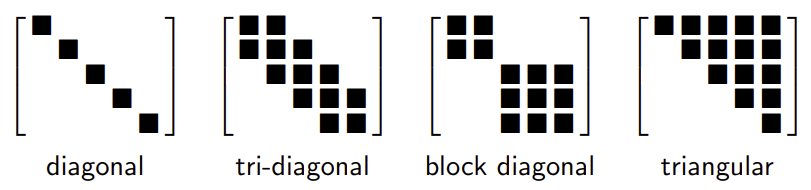
\includegraphics[width=.6\textwidth]{images/1.1}
\end{figure}

\subsubsection*{Matrix Transpose}
Transpose, denotes as $^T$, flips a matrix over is main diagonal, i.e. if $A$ is an $m \times n$ matrix then $A^T$ is an $n \times m$ matrix. It satisfies the following properties: 
\begin{itemize}
    \item $(A^T)^T = A$
    \item $(AB)^T = B^TA^T$
    \item $(A+B)^T = A^T + B^T$
\end{itemize}
If a matrix $A$ satisfies $A = A^T$ we say $A$ is \textbf{symmetric}. \par 
If a matrix $A$ satisfies $A = -A^T$ we say $A$ is \textbf{anti-symmetric}. \par 
Every square matrix $A$ can be written as the sum of a symmetric part and an anti-symmetric part: 
\[ A = \underbrace{\frac{1}{2}\left( A + A^T \right)}_{\text{symmetric}} + \underbrace{\frac{1}{2}\left( A - A^T \right)}_{\text{anti-symmetric}} \] 

\subsubsection*{Notation for Symmetric Matrices} 
We write 
\begin{itemize}
    \item $\mathbb{S}^n$ for the set of symmetric $n\times n$ matrices
    \item $\mathbb{S}^n_+ = \left\{ X \in \mathbb{S}^n \mid X \preceq 0 \right\}$ for the positive semi-definite $n\times n$ matrices  
    \[ X \in \mathbb{S}^n_+ \Leftrightarrow z^TXz \geq 0 \text{ for all } z. \] 
    \item $\mathbb{S}^n_{++} = \left\{ X \in \mathbb{S}^n \mid X \prec 0 \right\}$ for the positive definite $n\times n$ matrices 
\end{itemize}

\subsubsection*{Matrix Addition}
Two matrices of the same size can be added together: we simply add the corresponding elements in each matrix. 

\subsubsection*{Matrix Multiplication}
The product of two matrices $A \in \mathbb{R}^{m\times n}$ and $B \in \mathbb{R}^{n \times p}$ is an $m \times p$ matrix with elements 
\[ C_{ij} = \sum\limits_{k=1}^n A_{ik}B_{kj}. \] 

Matrix multiplication satisfies:
\begin{itemize}
    \item $(AB)C = A(BC)$ (associativity)
    \item $A(B+C) = AB + AC$ (left distributivity)
    \item $(A+B)C = AC + BC$ (right distributivity)
\end{itemize}
but matrix multiplication is not commutative: $AB \neq BA$ generally. \par 

\subsubsection*{Null Space}
The null space of a matrix $A \in \mathbb{R}^{m\times n}$ is defined as 
\[ \mathcal{N}(A) = \left\{ x \in \mathbb{R}^n \mid Ax = 0 \right\}. \] 
$\mathcal{N}(A)$ can be interpreted as
\begin{itemize}
    \item the set of all vectors mapped to zero by $y = Ax$
    \item the set of all vectors orthogonal to the rows of $A$
\end{itemize}
\subsubsection*{Range Space} 
The range space of a matrix $A \in \mathbb{R}^{m\times n}$ is defined as 
\[ \mathcal{R}(A) = \left\{ Ax \mid x \in \mathbb{R}^n \right\} \subseteq \mathbb{R}^m. \] 
$\mathcal{R}(A)$ can be interpreted as 
\begin{itemize}
    \item the set of all vectors that can be ``hit'' by $y = Ax$
    \item the span of the columns of $A$
    \item the set of all vectors $y$ such that $Ax = y$ has a solution
\end{itemize}

\subsubsection*{Orthogonal Complement}
The orthogonal complement of $V \subseteq \mathbb{R}^n$ is defined as 
\[ V^\perp = \left\{ x \mid z^Tx = 0 \text{ for all }  z\in V \right\}. \] 
We have $V \oplus V^\perp = \mathbb{R}^n$. \par

A result from the Fundamental Theorem of Linear Algebra states that $\mathcal{N}(A) = \mathcal{R}(A^T)^\perp$.

\subsubsection*{Rank}
The rank of a matrix $A \in \mathbb{R}^{m\times n}$ is 
\[ \mathrm{rank}(A) = \dim \mathcal{R}(A). \] 

\begin{itemize}
    \item $\mathrm{rank}(A) = \mathrm{rank}(A^T)$ 
    \item $\mathrm{rank}(A)$ is the maximum number of independent columns (or rows) of $A$. Hence $\mathrm{rank}(A) \leq \mathrm{min}\{m, n\}$. 
    \item $\mathrm{rank}(A) + \mathrm{dim}\mathcal{N}(A) = n$ (rank-nullity)
\end{itemize}
We say a matrix $A$ is \textbf{full rank} if $\mathrm{rank}(A) = \mathrm{min}\{m, n\}$. \par

The rank of the product of two matrices satisfies 
\[ \mathrm{rank}(AB) \leq \min\left\{ \mathrm{rank}(A), \mathrm{rank}(B) \right\}. \] 
If $A \in \mathbb{R}^{m\times n}$ has rank $r$ then $A$ can be factored as $BC$ with $B \in \mathbb{R}^{m\times r}$ and $C \in \mathbb{R}^{r \times n}$. 

\subsubsection*{Trace}
The trace of a square matrix $A \in \mathbb{R}^{n\times n}$ is the sum of its diagonal entries, i.e. 
\[ \mathrm{tr}(A) = \sum_{j=1}^n A_{jj}. \] 
Trace satisfies the following properties: 
\begin{itemize}
    \item $\mathrm{tr}(A) = \mathrm{tr}(A^T)$
    \item $\mathrm{tr}(\alpha A + \beta B) = \alpha\mathrm{tr}(A) + \beta\mathrm{tr}(B)$
    \item if $AB$ is square then $\mathrm{tr}(AB) = \mathrm{tr}(BA)$
\end{itemize}

\subsubsection*{Determinant}
The determinant of a square matrix $A \in \mathbb{R}^{n\times n}$ is a function $\det: \mathbb{R}^{n\times n} \rightarrow \mathbb{R}$ that satisfies the following properties:
\begin{itemize}
    \item $\det \bm{I} = 1$
    \item $\det \alpha A = \alpha^n \det A$
    \item swapping any two rows/columns changes the sign of the determinant 
    \item $\det AB = \det A \det B$
\end{itemize} 
We can interpret the determinant as the volume of the parallelepiped spanned by the rows (or columns) of $A$. \par

\subsubsection*{Matrix Inverse} 
The inverse of a square matrix $A \in \mathbb{R}^{n\times n}$ is a matrix $A^{-1}$ such that 
\[ AA^{-1} = A^{-1}A = \bm{I} \] 
A matrix is \textbf{invertible} (i.e. has an inverse) if and only if $\det A \neq 0$. This is equivalent to: 
\begin{itemize}
    \item the columns/rows of $A$ form a basis for $\mathbb{R}^n$
    \item $y = Ax$ has a unique solution for all $x \in \mathbb{R}^n$
    \item $A$ is full-rank (i.e. $\mathcal{N}(A) = \{ 0 \}$ and $\mathcal{R}(A) = \mathbb{R}^n$)
    \item $\det A^TA = \det AA^T \neq 0$
\end{itemize}

\subsubsection*{Cauchy-Schwarz Inequality}
For any vectors $x, y \in \mathbb{R}^n$, we have that 
\[ \abs{x^Ty} \leq \norm{x}_2 \norm{y}_2. \] 
The angle between vectors in $\mathbb{R}^n$ is given by 
\[ \theta = \cos^{-1}\left( \frac{x^Ty}{\norm{x}_2\norm{y}_2} \right). \] 
\begin{itemize}
    \item If $x$ and $y$ are aligned then $x^Ty = $
\end{itemize}

\subsubsection*{Eigenvalues and Eigenvectors}
$\lambda \in \mathbb{C}$ is an eigenvalue of $A \in \mathbb{R}^{n\times n}$ if 
\[ \det(\lambda I - A) = 0. \] 
Equivalently, there exists a non-zero $v \in \mathbb{C}^n$ such that $(\lambda I - A)v = 0$, or $Av = \lambda v$. Any such $v$ here is called an eigenvector of $A$, associated with eigenvalue $\lambda$. \par 
The eigenvalues of a symmetric matrix $A \in \mathbb{R}^{n\times n}$ are real. Moreover, there exists a set of orthogonal eigenvectors $q_1, \ldots, q_n$ such that $Aq_i = \lambda_iq_i$ and $q_i^Tq_j = 0$ if $i \neq j$. \par 
In matrix form, there is an orthonormal $Q$ such that $A = Q\Lambda Q^T$.

\subsubsection*{Norm Matrices}
A matrix norm is a function $\norm{\phantom{~.~}}: \mathbb{R}^{m\times n} \rightarrow \mathbb{R}$ that, similar to vector norms, satisfy linearity, positive definiteness, and the triangle inequality. \par
\begin{itemize}
    \item Induced norms: $\norm{A} = \sup \left\{ \norm{Ax} \mid x \in \mathbb{R}^n, \norm{x} \leq 1 \right\}$
    \item Frobenius norm: $\norm{A}_F = \sqrt{\left\{ \sum_{ij} a_{ij}^2 \right\}}$
    \item Nuclear norm: $\norm{A}_* = \sum_i \sigma_i(A) = \mathrm{tr}(\sqrt{A^TA})$  
\end{itemize} 
Square matrices also satisfy the sub-multiplicative property: 
\[ \norm{AB} \leq \norm{A}\norm{B}. \] 

\subsection{Matrix Factorization} 
\subsubsection*{LU Factorization} 
Every nonsingular matrix $A \in \mathbb{R}^{n\times n}$ can be factored as 
\[ A = PLU \] 
where $P$ is a permutation matrix, $L$ is unit lower triangular, and $U$ is upper triangular and non-singular. 
\subsubsection*{Cholesky Factorization} 
Every symetric positive definite matrix $A \in \mathbb{R}^{n\times n}$ can be factored as 
\[ A = LL^T \] 
where $L$ is lower triangular and non-singular with positive diagonal elements. 
\subsubsection*{Singular Value Decomposition} 
Any matrix $A$ can be decomposed as 
\[ A = U\Sigma V^T \] 
where $A \in \mathbb{R}^{m\times n}$ has rank $r$, $U \in \mathbb{R}^{m\times r}$, $V \in \mathbb{R}^{n\times r}$ which satisfy $U^TU = I$ and $V^TV = I$, and $\Sigma = \mathrm{diag}(\sigma_1, \ldots, \sigma_r)$ with $\sigma_1 \geq \sigma_2 \geq \cdots \geq \sigma_r > 0$. \par 
Since $A^TA = V\Sigma^2V^T$ we have $v_i$ are the eigenvectors of $A^TA$. Similarly, $u_i$ are the eigenvectors of $AA^T$. \par 
We can use SVD to interpret a linear map $y = Ax$ as follows: 
\begin{itemize}
    \item we compute coefficients of $x$ along the input directions $v_1, \ldots, v_r$
    \item scale the coefficients by $\sigma_i$
    \item re-constitute along the output directions $u_1, \ldots, u_r$
\end{itemize}
Here, $v_1$ is the most sensitive input direction, and $u_1$ is the highest gain output direction. 

\subsubsection*{Matrix Calculus}
We can compute partial derivatives of a function $f: \mathbb{R}^{m\times n} \rightarrow \mathbb{R}$ as 
\[ \pp[f(x)]{x_{ij}} = \lim_{\alpha \rightarrow 0} \frac{f(x + \alpha e_ie_j^T) - f(x)}{\alpha}. \] 
We can also compute the gradient (Jacobian) of $f$ as 
\[ \nabla_Af(A) = \begin{pmatrix}
    \pp[f]{A_{11}} & \pp[f]{A_{12}} & \ldots & \pp[f]{A_{1n}} \\
    \pp[f]{A_{21}} & \pp[f]{A_{22}} & \ldots & \pp[f]{A_{2n}} \\
    \vdots & \vdots & \ddots & \vdots \\
    \pp[f]{A_{m1}} & \pp[f]{A_{m2}} & \ldots & \pp[f]{A_{mn}} 
\end{pmatrix} \] 
Partial derivatives are linear: 
\begin{itemize}
    \item $\nabla_A(f + g) = \nabla_Af + \nabla_Ag$
    \item $\nabla_A(tf) = t\nabla_Af$
\end{itemize}
Chain rule and product rule also extend to matrix calculus. \par 
In vector calculus, the \textbf{Hessian} of a function $f: \mathbb{R}^n \rightarrow \mathbb{R}$ is the matrix of second-order partial derivatives of $f$, i.e. 
\[ \nabla_x^2 f(x) = \begin{pmatrix} 
    \pn*[f]{2}{x_1^2} & \pn*[f]{2}{x_1x_2} & \ldots & \pn*[f]{2}{x_1x_n} \\
    \pn*[f]{2}{x_2x_1} & \pn*[f]{2}{x_2^2} & \ldots & \pn*[f]{2}{x_2x_n} \\
    \vdots & \vdots & \ddots & \vdots \\
    \pn*[f]{2}{x_nx_1} & \pn*[f]{2}{x_nx_2} & \ldots & \pn*[f]{2}{x_n^2}
\end{pmatrix} \]  

\subsection{Probability Theory} 
A probability distribution is a function that maps outcomes of an experiment to probabilities: 
\begin{itemize}
    \item for discrete variables we have \textbf{probability mass functions} 
    \item for continuous variables we have \textbf{probability density functions} 
\end{itemize}
The \textbf{mean} or \textbf{expected value} of a random variable is the sum of possible values weighted by their probabilities: 
\[ \mathbb{E}[X] = \int_x x P(X = x) \di{x} \] 
The \textbf{variance} of a random variable $X$ is $\mathbb{E}[(X - \mathbb{E}[X])^2]$. \par 

\subsection{Geometric Concepts} 
\subsubsection*{Lines} 
A line through two points $x_1$ and $x_2$ has the equation $x = \theta x_1 + (1 - \theta) x_2$. \par 
The \textbf{line segment} between $x_1$ and $x_2$ is the set of points $x = \theta x_1 + (1 - \theta) x_2$ for $0 \leq \theta \leq 1$. \par

\subsubsection*{Affine Sets} 
An affine set contains the line through any two distinct points in the set: if $x_1, x_2 \in S$ then $\theta x_1 + (1-\theta) x_2 \in S$. \par 
Every affine set can be expressed as the solution set of a system of linear equations. 

\subsubsection*{Convex Sets} 
A convex set contains the line segment between any two distinct points in the set: if $x_1, x_2 \in S$ then $\theta x_1 + (1-\theta) x_2 \in S$ for $0 \leq \theta \leq 1$. \par
Common examples: 
\begin{itemize}
    \item nonnegative orthant: $\mathbb{R}_+^n$ = $\left\{ x \in \mathbb{R}^n \mid x_i \geq 0 \right\}$
    \item positive semidefinite matrices: $\mathbb{S}_+^n = \left\{ X \in \mathbb{R}^{n\times n} \mid z^TXz \geq 0, z \in \mathbb{R}^n \right\}$
\end{itemize}

\subsubsection*{Convex Combinations and Hulls} 
A convex combination of $x_1, \ldots, x_k$ is any point of the form 
\[ x = \theta_1x_1 + \theta_2x_2 + \ldots + \theta_kx_k \]
where $\theta_1 + \theta_2 + \ldots + \theta_k = 1$ and $\theta_i \geq 0$ for all $i$. \par
The convex hull of a set $S$, $\mathrm{conv}(S)$, is the set of all convex combinations of points in $S$. \par

\subsubsection*{Convex Cones} 
A \textbf{conic combination} of points $x_1$ and $x_2$ is any point of the form 
\[ x = \theta_1 x_1 + \theta_2 x_2 \] 
with $\theta_1, \theta_2 \geq 0$. \par 
A cone is a set containing all non-negative multiples of its points (i.e. if $x \in C$ then $\alpha x \in C$ for all $\alpha \geq 0$). \par
A convex cone is a set containing all conic combinations of its points. 

\subsubsection*{Hyperplanes and Halfspaces} 
A hyperplane is a set of the form $\left\{ x \mid a^Tx = b \right\}$ with $a \neq 0$. \par
A halfspace is a set of the form $\left\{ x \mid a^Tx \leq b \right\}$ with $a \neq 0$. \par
In the 3D case, a plane is a hyperplane while a halfspace is everything on one side of the plane. \par 
Hyperplanes are affine and convex, and halfspaces are convex.

\subsubsection*{Euclidean Balls and Ellipsoids} 
A Euclidean ball with center $x$ and radius $r$ is a set $B(x, r) = \left\{ y \mid \norm{y - x}_2 \leq r \right\}$. \par
An ellipsoid is a set of the form 
\[ \left\{ y \mid (y - x)^T P^{-1} (y - x) \leq 1 \right\} \] 
with $P \in \mathbb{S}_{++}^n$ (symmetric positive definite). \par 
Alternatively, we can represent a ball as 
\[ B(x, r) = \left\{ x + ru \mid \norm{u}_2 \leq 1 \right\} \] 
and an ellipsoid as 
\[ \left\{ x + Au \mid \norm{u}_2 \leq 1 \right\} \] 
with $A$ a square, nonsinguar matrix. 

\subsubsection*{Norm Balls and Cones} 
A norm ball with center $x$ and radius $r$ is the set $\left\{ y \mid \norm{y - x} \leq r \right\}$. \par 
A norm cone is the set $\left\{ (x, t) \mid \norm{x} \leq t \right\}$. 
Norm balls and cones are convex.

\subsubsection*{Polyhedra} 
A polyhedron is the solution set of finitely many linear inequalities and equalities 
\[ Ax \preceq b, Cx = d \] 
where $\preceq$ is componentwise inequality. \par 
So a polyhedron is the intersection of a finite number of halfspaces and hyperplanes. 
Polyhedra are convex sets. 

\subsubsection*{Summary of Convex Sets} 
\begin{figure}[H]
    \centering
    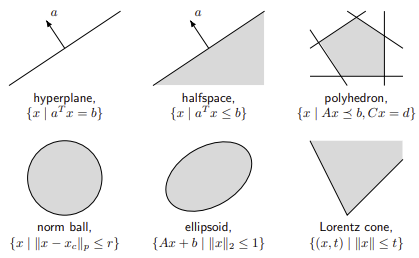
\includegraphics{images/2.1}
\end{figure}

\subsubsection*{Property of Convex Sets} 
We can either show a set $C$ is convex by applying the definition, or obtain $C$ using the following properties: 
\begin{itemize}
    \item the intersection of any number of convex sets is convex 
    \item the image of a convex set under an affine map is convex (recall affine maps are of the form $f(x) = Ax + b$)
    \item the preimage of a convex set under an affine map is convex
    \item perspective functions preserve convexity: these are functions of the form 
    \[ P(x, t) = x/t, t > 0 \] 
    \item linear-fractional functions preserve convexity: these are functions of the form 
    \[ f(x) = \frac{Ax + b}{c^Tx + d}, c^Tx + d > 0 \]     
\end{itemize}

\subsubsection*{Generalized Inequalities} 
A convex cone $K \subseteq \mathbb{R}^n$ is a \textbf{proper cone} if 
\begin{itemize}
    \item $K$ is closed (contains its boundary)
    \item $K$ is solid (has nonempty interior)
    \item $K$ is pointed (contains no line)
\end{itemize}
Examples include, 
\begin{itemize}
    \item the nonnegative orthant
    \item positive semidefinite cone $\mathbb{S}_+^n$
    \item nonnegative polynomials on $[0, 1]$ 
    \[ K = \left\{ x \in \mathbb{R}^n \mid x_0 + x_1t + x_2t^2 + \cdots + x_nt^n \geq 0, t \in [0, 1] \right\} \] 
\end{itemize}

A generalized inequality is a relation of the form 
\[ x \preceq_K y \Leftrightarrow y - x \in K \] 
and 
\[ x \prec_K y \Leftrightarrow y - x \in \mathrm{int}(K) \] 
where $\mathrm{int}(K)$ denotes the interior of $K$. \par 
\begin{itemize}
    \item In the case of the nonnegative orthant $K = \mathbb{R}^n_+$, we have componentwise inequality $x \preceq y \Leftrightarrow x_i \leq y_i$ for all $i$. 
    \item In the case of the positive semidefinite cone $K = \mathbb{S}_+^n$, we have $X \preceq Y \Leftrightarrow Y - X \in \mathbb{S}_+^n$.
\end{itemize}
In these cases, we omit the subscript $K$ and write $x \preceq y$ and $X \preceq Y$. \par

\subsubsection*{Minimum and Minimal Elements} 
As $\preceq$ is not a linear order, we have to define 
\begin{itemize}
    \item $x \in S$ is the minimum element of $S$ with respect to $\preceq$ if $x \preceq y$ for all $y \in S$
    \item $x \in S$ is the minimal element of $S$ with respect to $\preceq$ if there is no $y \in S$ such that $y \prec x$
\end{itemize}

\subsubsection{Separating Hyperplane Theorem} 
If $C$ and $D$ are nonempty disjoint convex sets, there exists $a \neq 0, b$ such that 
\[ a^Tx \leq b \text{ for } x \in C, \quad, a^Tx \geq b \text{ for } x \in D \] 
That is, there exists a hyperplane separating any two convex sets $C$ and $D$. (Strict separation requires additional assumptions, e.g. $C$ is closed, $D$ is singleton)
\subsubsection*{Supporting Hyperplane Theorem} 
A supporting hyperplane to a set $C$ at a boundary point $x_0$ is 
\[ \left\{ x \mid a^Tx = a^Tx_0 \right\}  \] 
where $a \neq 0$ and $a^T \leq a^Tx_0$ for all $x \in C$. \par
This can be thought of as a tangent hyperplane. \par 
The theorem states that there exists a supporting hyperplane at any point on the boundary of a convex set. \par 


\end{document}